\documentclass[a4paper, 11pt]{report}
\usepackage{graphicx}
\usepackage{subcaption}
\begin{document}

\section{parallel computing}
	\subsection{What is parallel computing}
The problem when facing large calculations is that they require a lot of computing power and time. Performing these calculations can be done in different types of computation but the most common ones are serial and parallel computation. Serial computing means, you have one compute unit (e.g. a single core CPU) available to deal with all the calculations that have to be done on a certain set of data. The problem will be broken into multiple smaller subproblems that will be solved by a certain instruction. The single compute unit has to perform the instruction on every subproblem to solve the main problem as shown in figure \ref{fig:SerialC}.
	\begin{figure}[h]
		\centering
		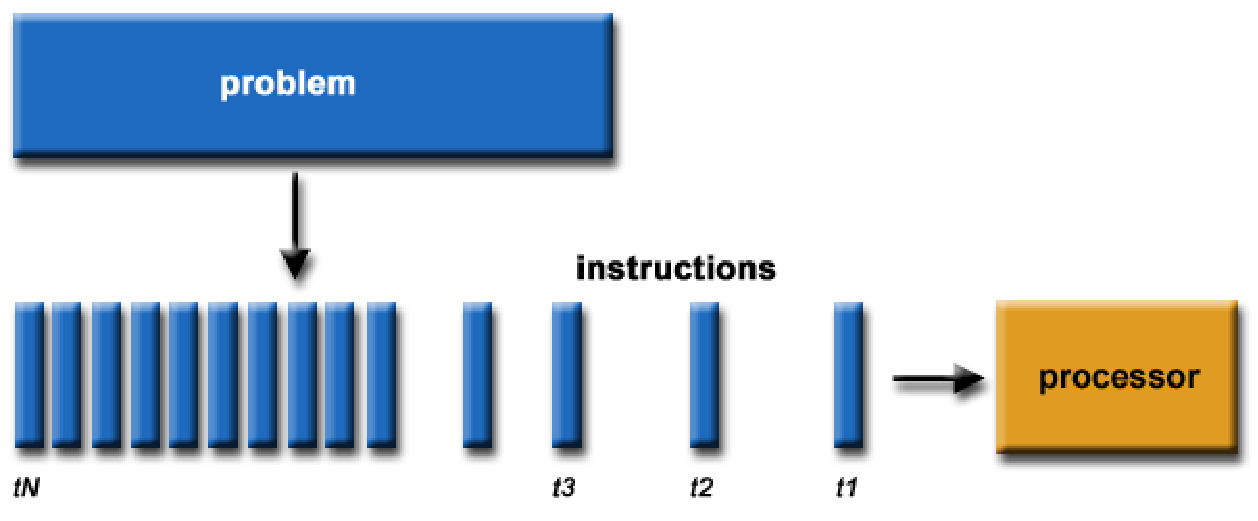
\includegraphics[scale=.4]{images/serialProblem.pdf}
		\caption{Workflow serial computing}
		\label{fig:SerialC}
	\end{figure}

Parallel computing, on the other hand, is the simultaneous use of multiple compute units (CPU+GPU), or a compute resource, to solve a computational problem. We break apart the main problem in smaller subproblems as we did with serial computing. Each part is further broken down to a series of instructions again.Now, since there are multiple compute units, we can distribute the subproblems among all these compute units. Every unit can now perform the instruction on their given subproblems simultaneously as shown in figure \ref{fig:ParallelC}. One compute resource can constist of multiple compute units, for example it can include multiple processors or it's just a number of computers connected by a network.
	\begin{figure}[h]
		\centering
		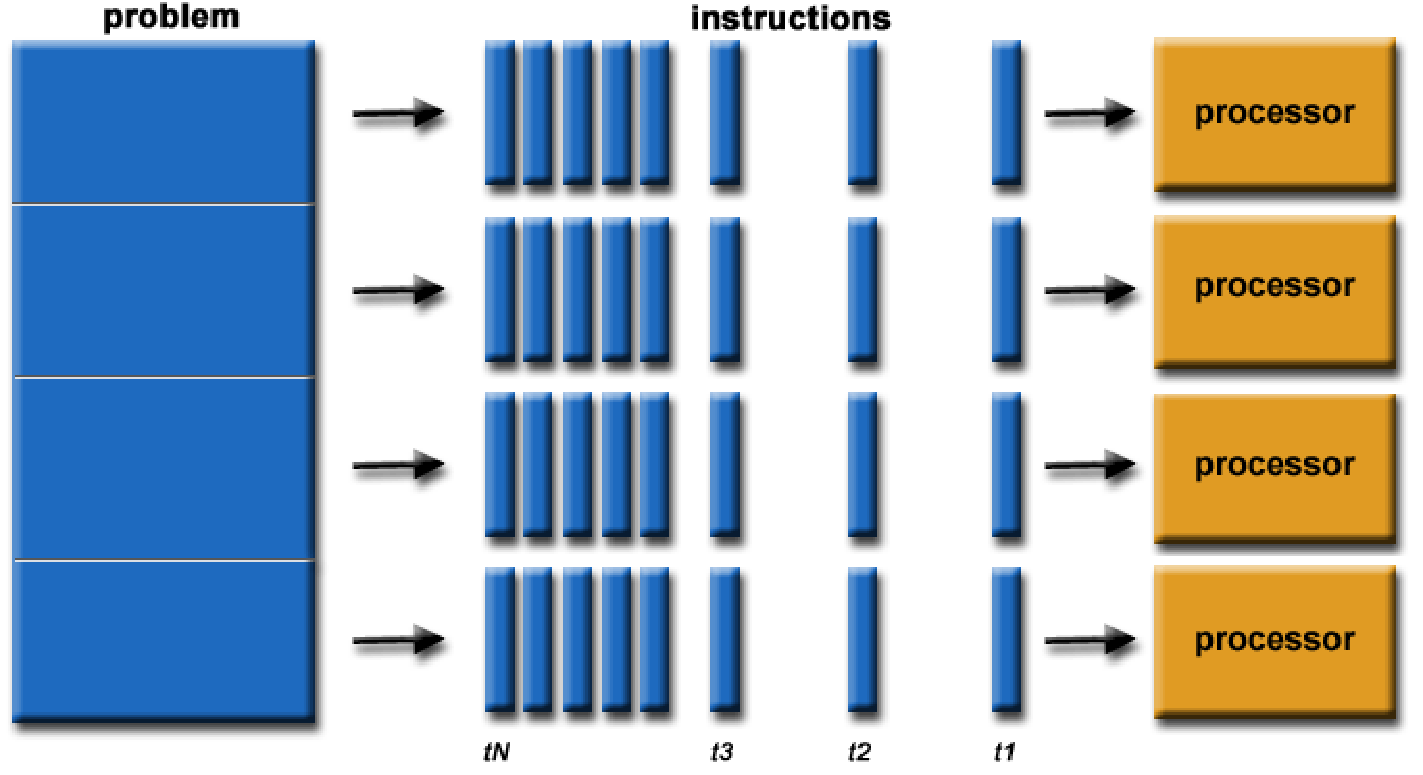
\includegraphics[scale=.4]{images/parallelProblem.pdf}
		\caption{Workflow parallel computing}
		\label{fig:ParallelC}
	\end{figure}
With multiple compute units for one task, we will shorten the completion time aswell have potential cost savings. It also allows us to solve larger/complex problems since a single computer could suffer from limited memory. And last, we are able to access non-local resources in a network that wouldn't be accessable from a local computer.

It is easy to conclude that the concept of parallel computing was to have a more efficient way to handle with large sets of data such as images or simulations that involve multiple parameters. It's also easier to handle with complex data for example in algorithms \cite{barney2012parallel}.

	\subsection{Classification of parallel computing}
Parallel computing systems can be seperated into different classes. According to Flynn's taxonomy, we can roughly place any of these systems in one of the four classes he defined. This classification was first studied and proposed by Michael Flynn in 1972 \cite{Unit2COPC}. The classifications are determined by two factors: instruction stream and data stream which both have two possible states being single or multiple. Figure \ref{fig:flynnTaxonomy} represents a matrix of the four possible classes from the Flynn's taxonomy \cite{barney2012parallel}.

	\begin{figure}[h]
		\centering
		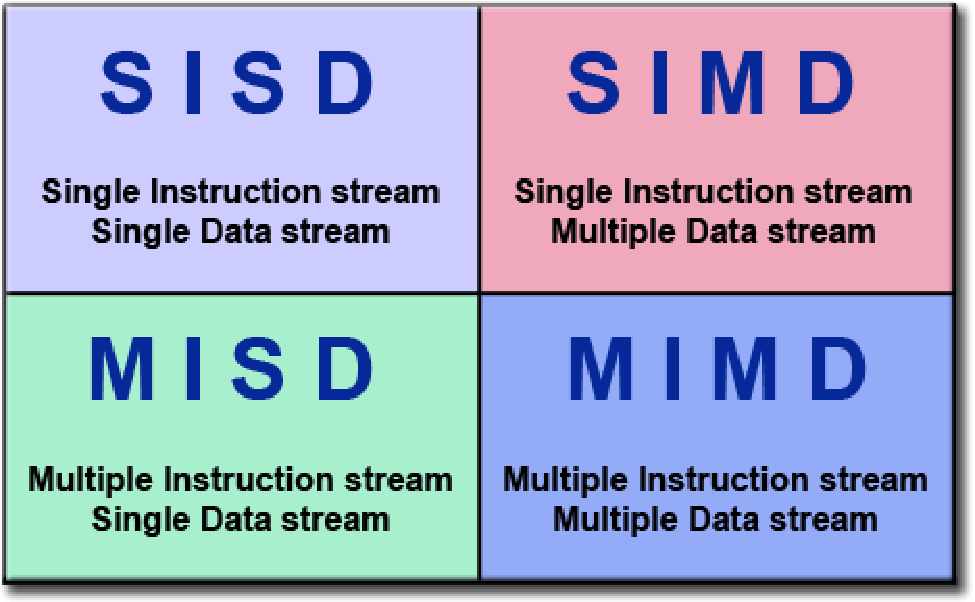
\includegraphics[scale=.5]{images/flynnsTaxonomy.pdf}
		\caption{Four possible classifications according to Flynn's Taxonomy}
		\label{fig:flynnTaxonomy}
	\end{figure}
	
	\begin{itemize}
		\item SISD
	\end{itemize}
The SISD class will have a single processor executing a single data stream to operate on data stored in a single memory (figure \ref{fig:sisd}). This means that a parallel compute system cannot be classified as an SISD sytem, but Flynn's taxonomy wasn't made for just classifying parallel compute systems. It's usually old computers and other older compute units that can be classified as SISD.
	
	\begin{itemize}
		\item SIMD
	\end{itemize}
Data is disctributed amongst multiple processors who all execute the same instruction (figure \ref{fig:simd}). Since we have access to multiple compute units, parallel computing can be categorized in this class. Furthermore, this is the class where we can categorize our subject of the thesis in since we have a large set of data divided over multiple data streams (MD) and only one instruction stream (SI) since all processing units will perform the same instruction on the data. The SIMD class contains most modern computers, particularly those with a graphics processor unit (GPU).

	\begin{itemize}
		\item MISD
	\end{itemize}
Each processing unit operates on the data independently via separate instruction streams while a single data stream is fed into multiple processing untis (figure \ref{fig:misd}). This class knows very few applications. An example of an application is the use of multiple cryptography algorithms attempting to crack a single coded message.
	
	\begin{itemize}
		\item MIMD
	\end{itemize}
This time every processing unit is able to execute a different instruction stream on a different data stream (figure \ref{fig:mimd}). This means that any instruction can be applied on any data package for every compute unit. Most supercomputers, networked parallel computer clusters and "grids" can be classified as a MIMD compute system. Also, many MIMD architectures include SIMD execution sub-components.

\begin{figure}[h]
	\centering
	\begin{subfigure}[t]{0.4\textwidth}
		\centering
		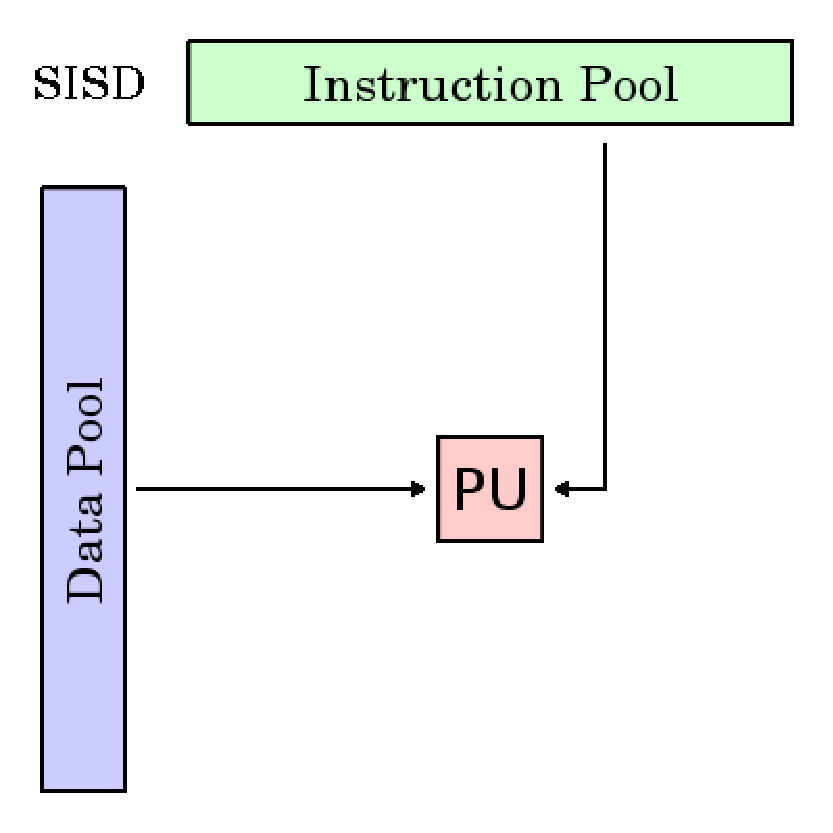
\includegraphics[scale=.3]{images/sisd.pdf}
		\caption{SISD}\label{fig:sisd}
	\end{subfigure}
	\begin{subfigure}[t]{0.4\textwidth}
		\centering
		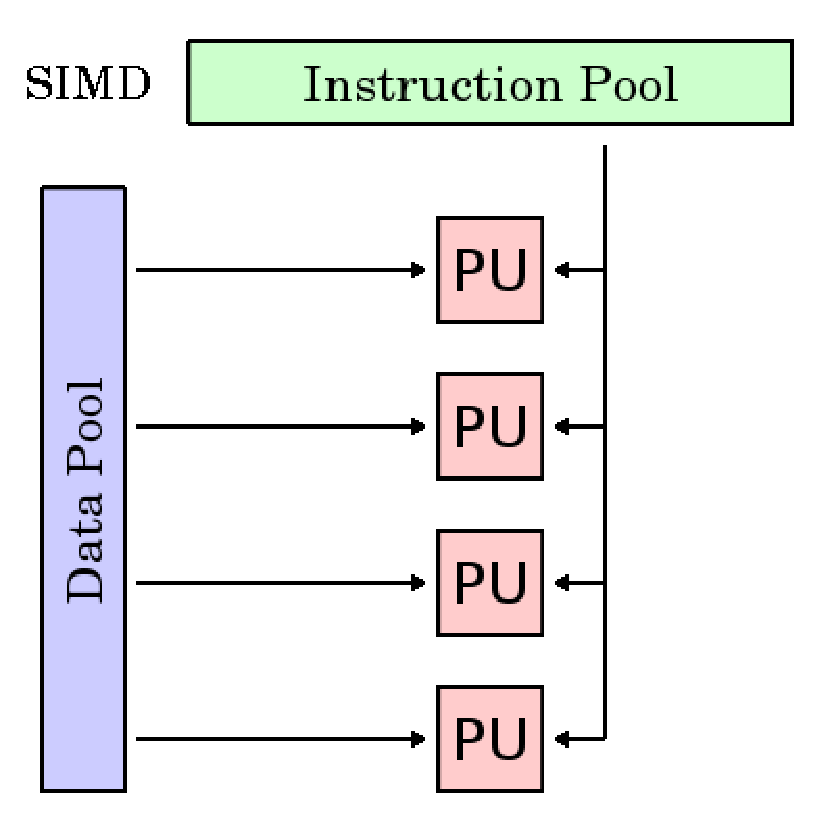
\includegraphics[scale=.3]{images/simd.pdf}
		\caption{SIMD}\label{fig:simd}
	\end{subfigure}
	\begin{subfigure}[t]{0.4\textwidth}
		\centering
		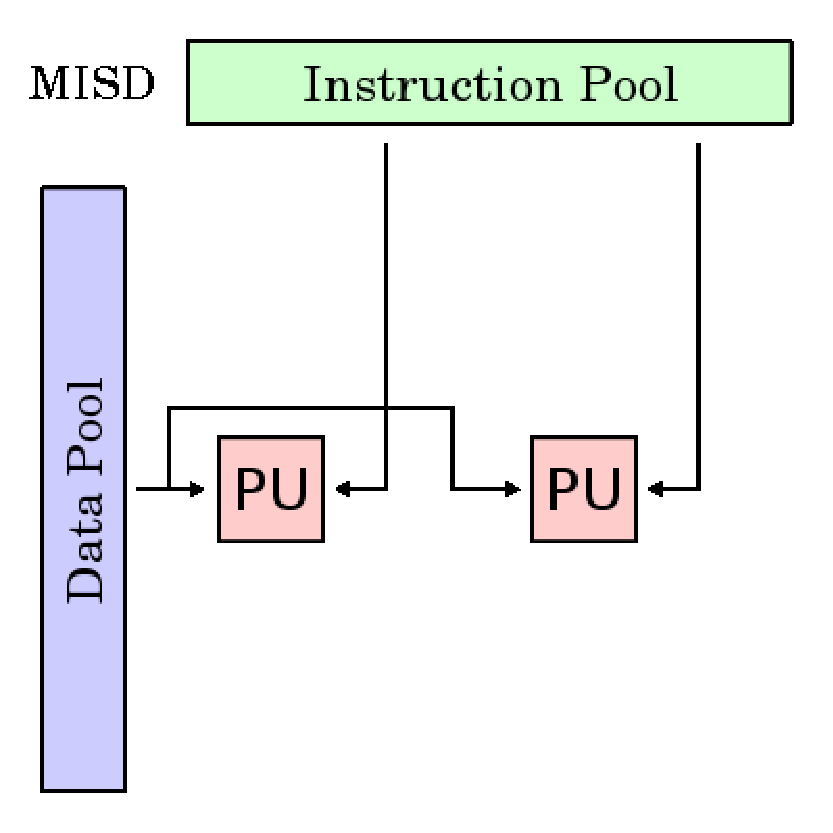
\includegraphics[scale=.3]{images/misd.pdf}
		\caption{MISD}\label{fig:misd}
	\end{subfigure}
	\begin{subfigure}[t]{0.4\textwidth}
		\centering
		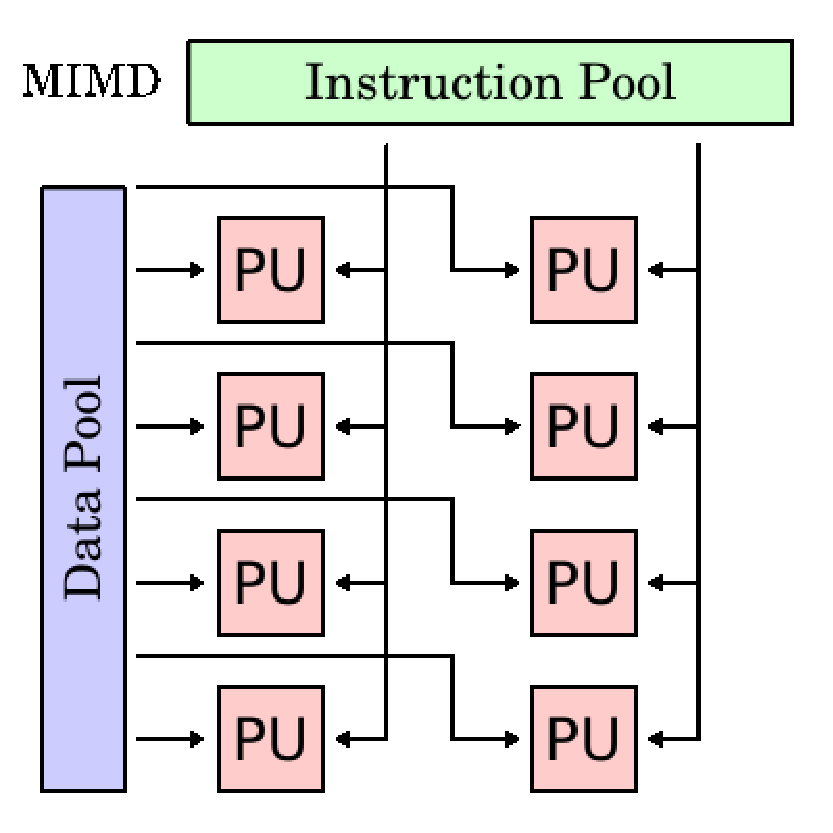
\includegraphics[scale=.3]{images/mimd.pdf}
		\caption{MIMD}\label{fig:mimd}
	\end{subfigure}
	\caption{Architecture classes from Flynn's taxonomy}\label{fig:archFlynnTax}
\end{figure}

	\subsection{Amdahl's law}
Amdahl's Law can be used to theoretically calculate how much a computation can be sped up by running part of it in parallel, versus using only one serial processor \cite{amdahlslaw}. A program can be split up in two parts, a part that cannot be parallelized (A) and a part that can be parallelized (B). The speedup factor S for both parts can be calculated by dividing the execution time for serial computation T(1) by the execution time for parallel computation T(j), with j the amount of processing units.
\begin{equation}
	S = \frac{T(1)}{T(j)}
\end{equation}
Since A is a serial computation, the amount of processing units j equals 1. And thus the speedup factor for A is also 1. Part A can only be executed faster by optimizing the code. Let's call this optimization factor O. For part B, we define the number of compute units by N. The total execution time then equals:
\begin{equation}
	T = \frac{A}{O} + \frac{B}{N}	
\end{equation}
Part B can also be interpreted as the total program minus part A. Note that non-parallelizable part A benefits from the optimization mentioned earlier:
\begin{equation}
	B = \frac{1-A}{O}
\end{equation}
The total execution time T with variables O and N then equals:
\begin{equation}
	T(0, N) = \frac{A}{O} + (\frac{1-A}{O})/N
\end{equation}
The total program speedup S can be calculated with Amdahl's law by comparing the execution time of the old program T with the execution time of the new program T(O, N):
\begin{equation}
	S  = \frac{T}{T(O, N)}
\end{equation}


\section{OpenCL}\label{subsec:OpenCL}
	
\section{Bluetooth}
Bluetooth is a form of wireless communication and was developed in 1994 by L. M. Ericsson of Sweden. It is a radio frequency (RF) technology using the 2.4GHz industrial, scientific and medical (ISM) band, the same band where you can find ZigBee and WiFi aswell. It can be used to transmit data or voice communication over short-distances. Bluetooth radios can be found in nearly every new smartphone and laptop device. It's easy to use, to setup and it has a lot of applications, for example home heating systems, entertaining devices and so on. Bluetooth is designed to be low cost, for about 10\$ per unit. The down side of this, is the short connection range and the limited transmission speed of around 780 kb/s\cite{bluetoothTech}.\\

	\subsection{Bluetooth benefits}
The introduction of bluetooth allowed for many new appliacations in several areas. Even today it is still widely used, mostly for multimedia devices, smartwatches, keyboards, mices, printers. The following list explains some benefits for three general areas for Bluetooth:
		\paragraph{Data and voice acces points.}
Bluetooth allows a wireless connection between devices through which they can communicate. With Bluetooth, the devices are able to trasmit voice and data packages in real-time.
		\paragraph{Cable replacement.}
Some wired connections between devices require special cables or adapters. Bluetooth eliminates this hastle since any device can connect to another with the right communication protocol. The range of this connection is approximately 10m and doesn't require the devices to be in line of sight. With an optional amplifier the range can be extended to 100m.
		\paragraph{Ad hoc networking.}
Devices with a bluetooth radio can establish instant connections with each other as soon they come into range.


	\subsection{Master, slave and piconet}
For a Bluetooth connection to exist, their has to be atleast one master and one slave device. They use what is called the master/slave model. A master device can be connected to up to seven slave devices while a slave can only connect to one master device. A network of one master and one to seven slaves is called a piconet. The master device will coordinate all the communication throughout the piconet. All slave devices are allowed to exchange data with the master device when granted premission, but can't communicate with other slaves in the piconet. The connection between each device is encoded and protected to prevent other devices from eavesdropping and to prevent interference between other devices. Furthermore, in order for these devices to connect with each other, they require the same communication protocol. A device in one piconet can also exist as part of another piconet and can function as either a slave or a master in each piconet. This form of overlapping is called a scatternet \cite{introBluetooth}. An example of two piconets forming a scatternet is shown in figure \ref{fig:scatternet}.

\begin{figure}[h]
	\centering	
	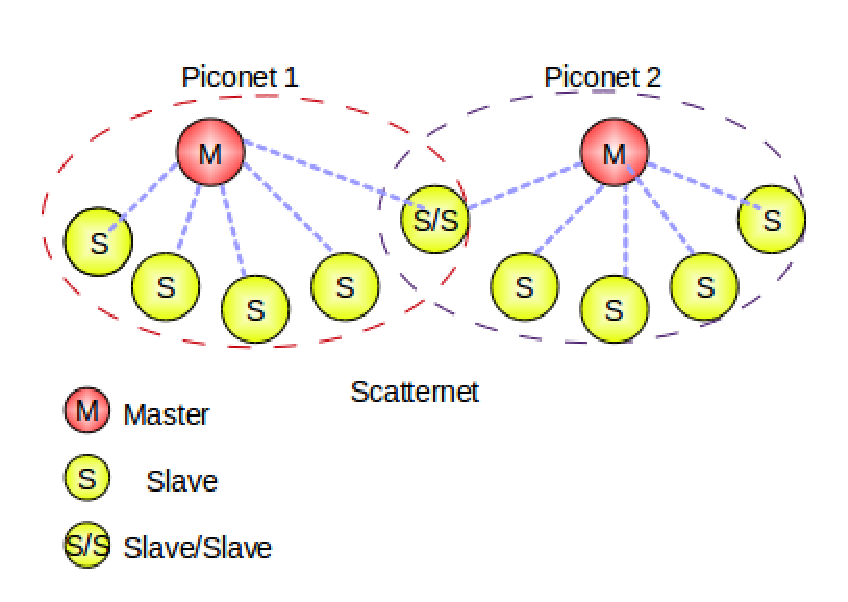
\includegraphics[scale=0.60]{images/scatternet.pdf} 
	\caption{Piconets and Scatternets}\label{fig:scatternet}
\end{figure}

The piconet/scatternet allows the devices to share the same physical area, allowing the network to make an efficient use of the bandwidth. A Bluetooth system can use up to 79 different frequencies using a frequency hopping (from 2.402 to 2.480 GHz) \cite{bluetoothStack} scheme with a carrier spacing of 1MHz. This allows a bandwidth of 80MHz. Without frequency hopping scheme, every single channel would have a bandwidth of 1MHz at their disposal. With frequency hopping, the sequence will define a logical channel. This allows to have an available bandwidth of 1MHz at any given time, with a maximum of eight devices sharing the bandwidth. This 80 MHz bandwidth can be shared by several different logical channels. Though, this can cause signal collisions when devices in different piconets, on different logical channels have the same hop frequency at a given time. Signal collisions degrade the performance, so we can state that the more piconets we have, the more collisions occur, the lower our total performance will be \cite{introBluetooth}.

	\subsection{Protocol architecture}
The bluetooth protocol architecture consists of four basic layers: core protocols, cable replacement, telephony control protocols and adopted protocols. Figure \ref{fig:bluetoothStack} shows the architecture of the Bluetooth protocol stack.
\begin{figure}[h]
\centering
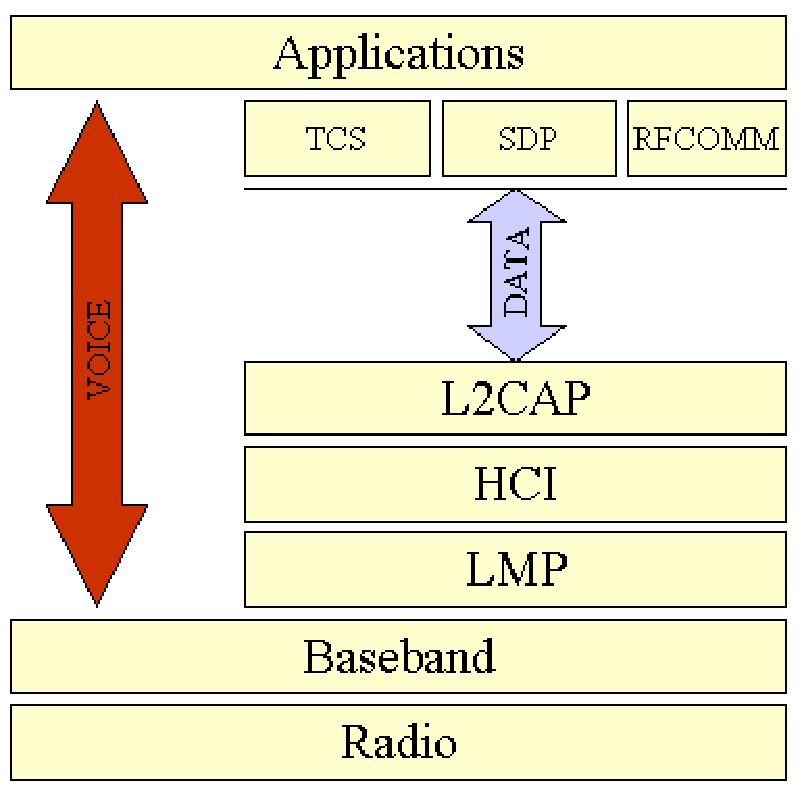
\includegraphics[scale=0.5]{images/bluetoothStack.pdf}
\caption{Bluetooth protocol stack}\label{fig:bluetoothStack}
\end{figure}


		\paragraph{Core protocols.}
The core protocol is a five-layer stack. Every layer in the stack has its own responibilites that are mentioned below.

\begin{itemize}
		\item The \textit{radio} layer is the wireless connection that specifies certain details about the air interface, including frequency, the use of frequency hopping, modulation scheme and transmit power. 
		\item The \textit{baseband} layer is responsible for the packet transmission to the radio layer. As mentioned before these packet can contain data or voice. For the data packages, asynchronous connectionless (ACL) links are used while voice packages are transmitted with synchronous connection-oriented (SCO) links. The baseband layer maintains both ACL and SCO links. It is important for data packages to be transmitted correctly to maintain data integrity, while it is not a problem in case some voice packages get lost. That is why SCO packages are never retransmitted. If you would retransmit voice packages, every next package would suffer from a time delay restraining us from having real-time communication.
		\item The \textit{Link manager protocol (LMP)} uses the links setup by the baseband and manages the connection between Bluetooth devices. Furthermore, it is responsible for monitoring service quality, security aspects such as device authentication, encryption plus the control and negotiation of baseband packet sizes.
		\item The \textit{Host controller interface (HCI)} is the layer between the hardware and the software. The L2CAP layer and the layers above it are implented in the software while all other layers under the HCI (LMP, baseband, radio) are part of the hardware. the HCI driver acts as a physical bus that connects the hardware with software. It is possible to access the L2CAP layer directly by the application making it easier for application programmers. This makes the HCI an unnecessary component in some cases.
		\item The \textit{Logical link control and adaptation protocol (L2CAP)} receives application data and transforms this to the Bluetooth format. Furthermore, Quality of Service (QoS) parameters are exchanged at this layer \cite{bluetoothStack}.
		\item According to \cite{bluetoothStack}, the \textit{Service discovery protocol (SDP)} is not a part of the Core protocols. Though, it contains all the information, services and charasteristics  in order to establish a connection between two or more bluetooth devices. The LMP uses the SDP's first to find out what services are available from the acces point. Then information from the SDP is obtained by the LMP to create a L2CAP channel.
\end{itemize}
		
	\paragraph{Cable replacement.}
The RFCOMM seen in figure \ref{fig:bluetoothStack} is the cable replacement protocol. It is a virtual serial port that is designed to replace cable technology. Serial ports are common types of communication interfaces used with computing ang communication devices \cite{introBluetooth}. So with RFCOMM we eliminate the need for serial ports for communication between two devices, assuming both are equiped with a Bluetooth radio.


\section{Websocket server}

\bibliographystyle{IEEEtran}
\bibliography{References}
\end{document}
